\section{Teilkonzepte}
In diesem Abschnitt werden die Teilkonzepte der evaluierten Lösungsvariante \glqq Frosch\grqq{} beschrieben. Es werden Konzepte zu den einzelnen Funktionen erstellt. Abschliessend wird das Zusammenspiel der Teilkonzepte anhand eines Blockschaltbild erklärt.

TODO Gesamtkonzeptvisualisierung

\subsection{Treppensteigen}

\begin{figure}[H]
  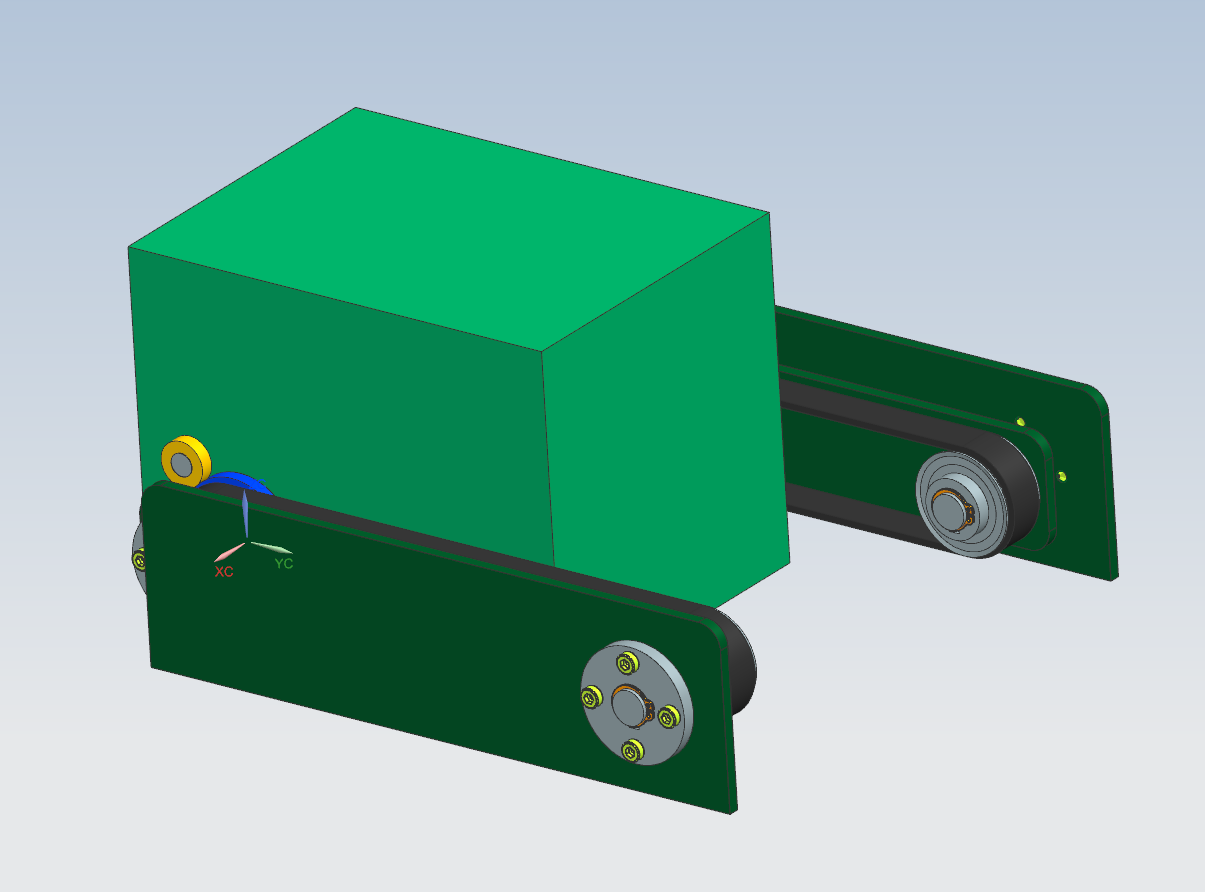
\includegraphics[width=1\textwidth]{img/Treppensteigen/Geraetansicht.PNG}
  \centering
  \caption{Visualisierung Treppensteigkonzept}
\end{figure}

\newpage

% TODO: Korrekturlesen Treppensteigen

\subsubsection{Funktionsprinzip}
Für das Treppensteigen wird die Variante \glqq Frosch \grqq{} evaluiert. Der Grundkörper des Gerätes, in dem Antriebe, Steuerung, Energieversorgung und Orientierungskomponenten enthalten sind, wird auf beiden Seiten mit jeweils einem Standfuss und einer Verbindungsleiste erweitert. Von der Drehachse 1 zur Drehachse 2 wird ein Zahnriemen gespannt. Mit diesen zusätzlichen Elementen soll die Treppe bestiegen werden.

\begin{figure}[H]
  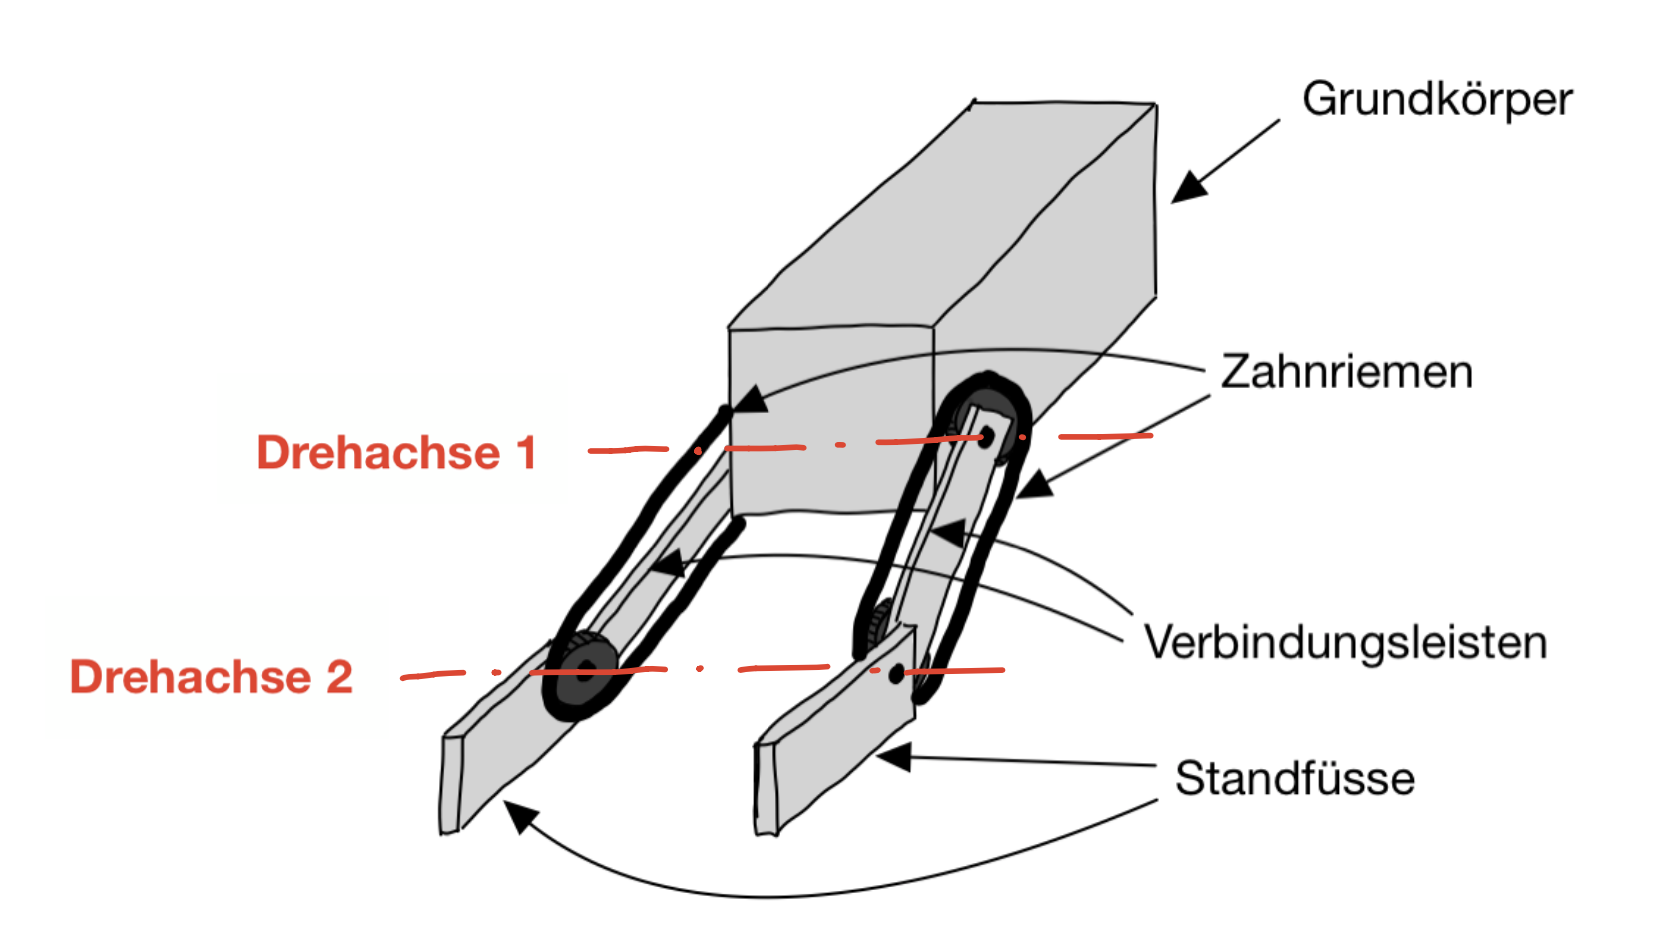
\includegraphics[width=1\textwidth]{img/Treppensteigen/Skizze Drehachsen.png}
  \centering
  \caption{Skizze Drehachsen}
\end{figure}

Eine Treppenstufe soll mit zwei Hubbewegungen erklommen werden. In einer ersten Hubbewegung bleiben die Standfüsse auf der letzten Stufe und der Grundkörper wird auf die nächste Stufe gehoben. Bei dieser Bewegung soll der Grundkörper horizontal gehalten werden.

\begin{figure}[H]
  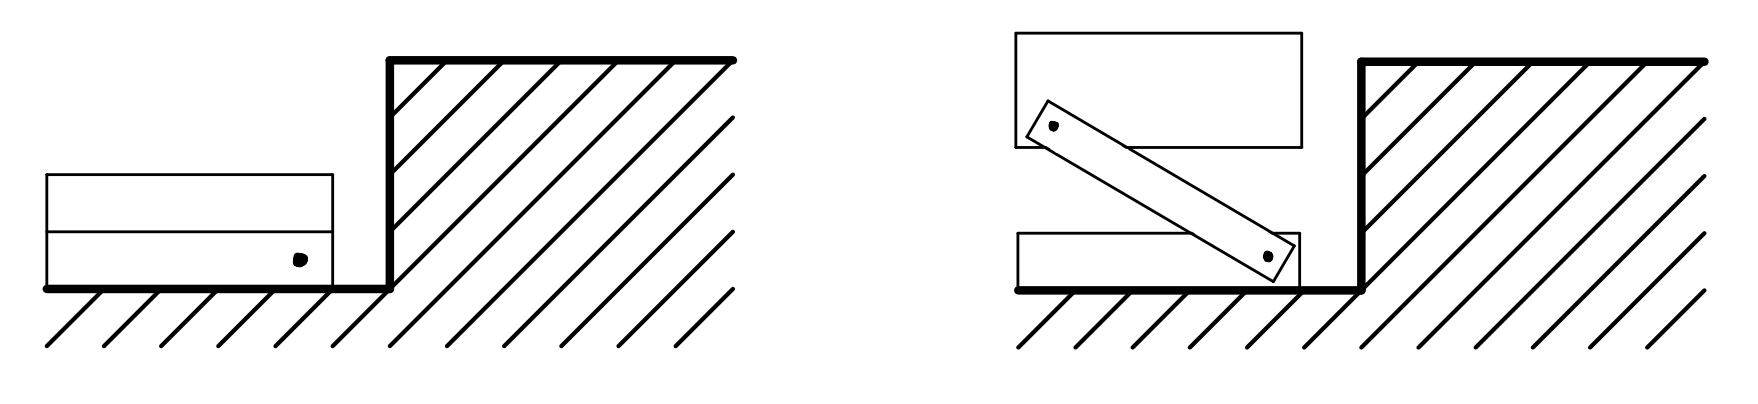
\includegraphics[width=1\textwidth]{img/Treppensteigen/1. Hubbewegung Skizze.png}
  \centering
  \caption{Skizze 1. Hubbewegung}
\end{figure}
 
 
Bei der zweiten Hubbewegung müssen die Standfüsse auf die nächste Treppenstufe, zurück an die Seiten des Grundkörpers geholt werden.

\begin{figure}[H]
  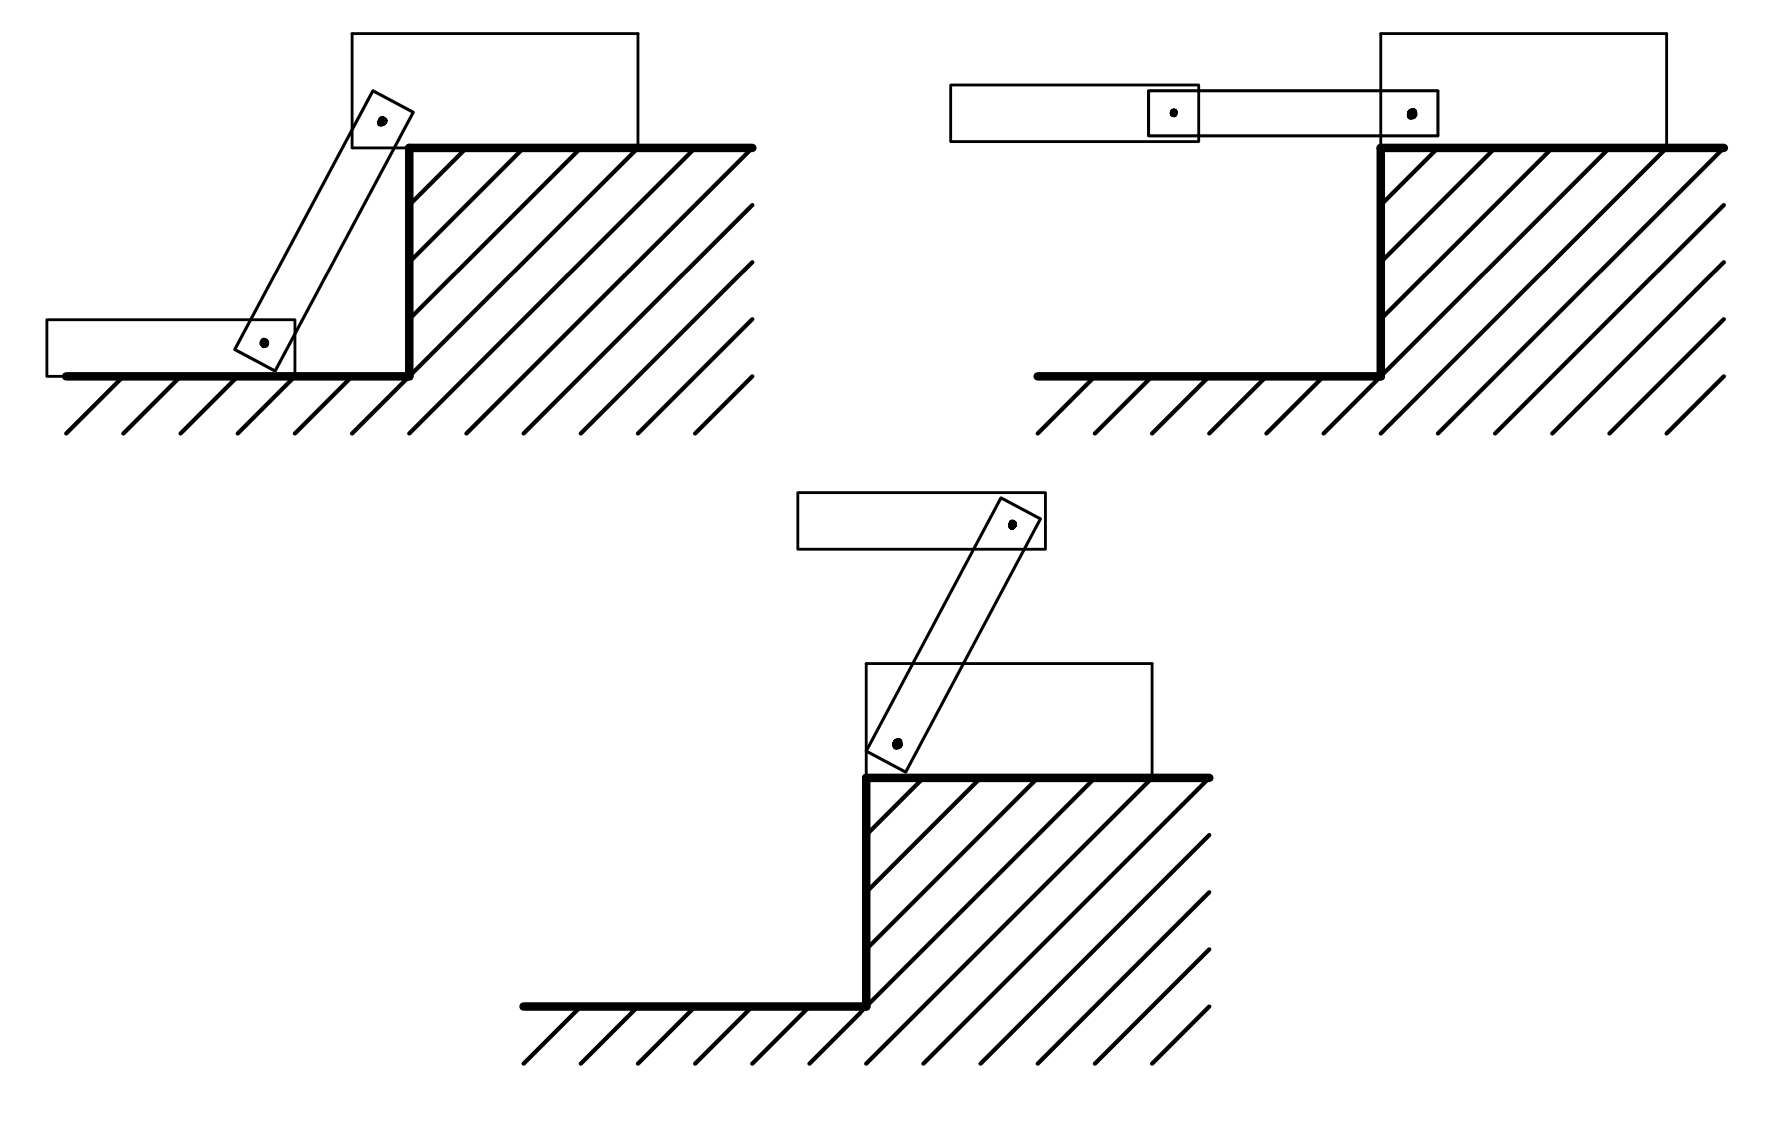
\includegraphics[width=1\textwidth]{img/Treppensteigen/2. Hubbewegung Skizze.png}
  \centering
  \caption{Skizze 2. Hubbewegung}
\end{figure}
 
\newpage

\subsubsection{Funktionen der Komponenten}

\textbf{Drehachse 1}

Die Verbindungsleisten sind über eine Welle (Welle 1) mit dem Grundkörper verbunden (Drehachse 1). Die Verbindungsleisten sind fest auf der ersten Welle fixiert, sodass bei einer Drehung der Welle sich die Verbindungsleisten um den gleichen Winkel drehen. Das Antriebsrad des Zahnriementriebes ist lose auf der ersten Welle montiert, sodass die Drehbewegungen der Welle und des Antriebsrads des Zahnriemens unabhängig sind.
\\


\textbf{Drehachse 2}

Die Verbindungsleisten sind mit den Standfüssen bei der zweiten Drehachse verbunden. Die zweite Drehachse ist nicht eine Drehachse, sondern auf beiden Seiten eine einzelne Drehachse. Sie sind aber immer gleich ausgerichtet und werden als eine Drehachse betrachtet (Drehachse 2). Die Standfüsse sind mit den Verbindungsleisten auf beiden Seiten einzeln über kleine, kurze Wellen (Welle 2) verbunden. 

Bei der zweiten Drehachse muss auf beiden Seiten ein Moment aufgebracht werden für die erste Hubbewegung, damit sich die Standfüsse und Verbindungsleisten gegeneinander bei der zweiten Drehachse verdrehen und so der Grundkörper nach oben gehoben wird. Das Moment bei den zweiten Drehachsen kann nicht direkt mit einzelnen, zwei an die Wellen 2 gekoppelten Motoren angetrieben werden, da die Motoren bei den Hubbewegungen im Weg wären, wenn sie an den Innenseiten angebracht würden oder die Kabel der Motoren wären im Weg bei einer Aussenmontur. Aus diesem Grund muss das Moment für die erste Hubbewegung von der ersten Welle auf die kleinen, kurzen Wellen auf beiden Seiten übertragen werden. Für diese Übertragung des Drehmomentes mit einem grossen Achsabstand eignen sich Zugmittelgetriebe wie Ketten-, Riementriebe. Da das Gewicht nicht zu gross werden soll, kommen Ketten nicht in Frage. Da das Drehmoment in einem gewissen Verhältnis und ohne Schlupf übertragen werden soll, eignet sich ein Zahnriemen am besten. Bei der zweiten Welle sind die Standfüsse mit dem Abtriebsrad des Zahnriementriebes gekoppelt und machen so die gleichen Drehbewegungen. Weiter sind bei der zweiten Drehachse die Standfüsse nicht mit den Verbindungsleisten gekoppelt, da sie sich zueinander verdrehen müssen, um die Hubbewegungen auszuführen.

\newpage

\textbf{Hubbewegungen}

Für die erste Hubbewegung wird an den Antriebszahnriemenrädern ein Moment eingeleitet. Die Antriebszahnriemenräder sollen je mit einem Zahnrad verbunden werden. Mit einer Übersetzung soll ein erster Elektrogetriebemotor (Motor 1) über eine zusätzliche Welle diese Antriebszahnriemenräder antrieben. Um den Grundkörper bei der ersten Hubbewegung horizontal halten zu können soll auf der ersten Welle ein Zahnrad angebracht werden, um mit einem zweiten Elektrogetriebemotor (Motor 2) das Moment der Gewichtskraft des Grundkörpers auszugleichen.

Bei der zweiten Hubbewegung wird die Drehung der Standfüsse bei der zweiten Drehachse mit dem ersten Motor(Motor 1) kontrolliert. Die Drehung der Verbindungsleisten bei der ersten Drehachse wird vom zweiten Motor angetrieben. Mit diesem Aufbau ist es möglich die Standfüsse einzeln zu verdrehen. Somit kann das nötige Drehmoment verkleinert werden, wenn bei der zweiten Hubbewegung die Standfüsse nicht horizontal gehalten werden.


\subsubsection{Erste Abmasse}

Anhand der vorgegebenen Treppe wurden erste Massabschätzungen gemacht. Dabei wurde die Tritthöhe und die Tritttiefe berücksichtigt.

\begin{figure}[H]
  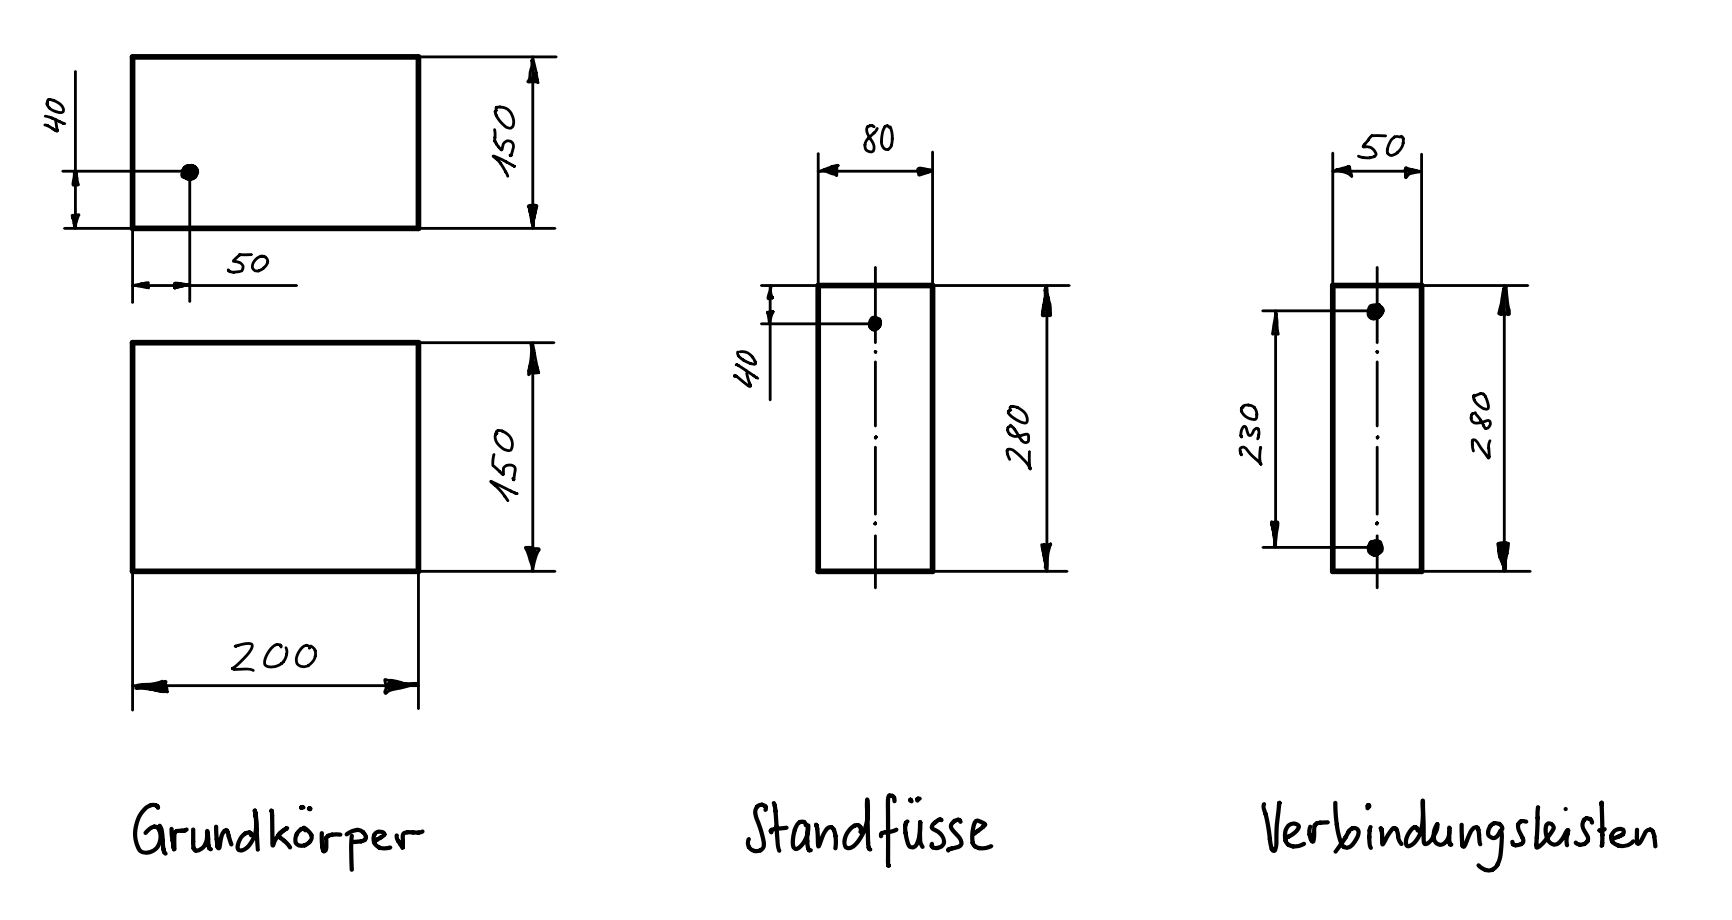
\includegraphics[width=1
  \textwidth]{img/Treppensteigen/Erste Abmasse}
  \centering
  \caption{Skizze erste Abmasse}
\end{figure}

\newpage

\subsubsection{Standsicherheit}

Mit den ersten Massabschätzungen wurde eine erste Standsicherheitsbetrachtung bei den zwei Hubbewegungen gemacht. Dabei wurde das Wunschgewicht, dass in der Anforderungsliste definiert wurde verwendet. Die Standfüsse und die Verbindungsleisten sollen aus Aluminium mit einer Dichte\cite{Aluminium} von 2.7 g/cm$^{3}$ sein. Ihr Gewicht wurde mit den ersten Massabschätzungen berechnet.


\textbf{Berechnung Masse Standfüsse:}

Material: Aluminium

Dicke t: 5 mm

\(\rho_{Aluminium} = 2.7\ g/cm^3\)

\[V_{1 Standfuss} = a\ *\ b\ *\ t\ = 280\ mm\ *\ 80\ mm\ *\ 5\ mm = 112\ cm^3\]

\[m_{1 Standfuss} = V_{1 Standfuss} * \rho_{Aluminium} = 112 cm^3 * 2.7 g/cm^3 = 0.3\ kg\]

\[m_{2 Standfuesse} = 2\ *\ m_{1 Standfuss} = 0.6\ kg\]


\textbf{Berechnung Masse Verbindungsleisten:}

Material: Aluminium

Dicke t: 5 mm

\(\rho_{Aluminium} = 2.7\ g/cm^3\)

\[V_{1 Verbindungsleiste} = a\ *\ b\ *\ t\ = 280\ mm\ *\ 50\ mm\ *\ 5\ mm = 70\ cm^3\]

\[m_{1 Verbindungsleiste} = V_{1 Verbindungsleiste} * \rho_{Aluminium} = 70 cm^3 * 2.7 g/cm^3 = 0.2\ kg\]

\[m_{2 Verbindungsleisten} = 2\ *\ m_{1 Verbindungsleiste} = 0.4\ kg\]

\newpage

\textbf{1.Hubbewegung:}\\

m$_{ges}$ = 3kg

m$_{Grundkoerper}$ = 2 kg

m$_{Standfuesse}$ = 0.6 kg

m$_{Verbindungsleisten}$ = 0.4 kg\\

\begin{figure}[H]
  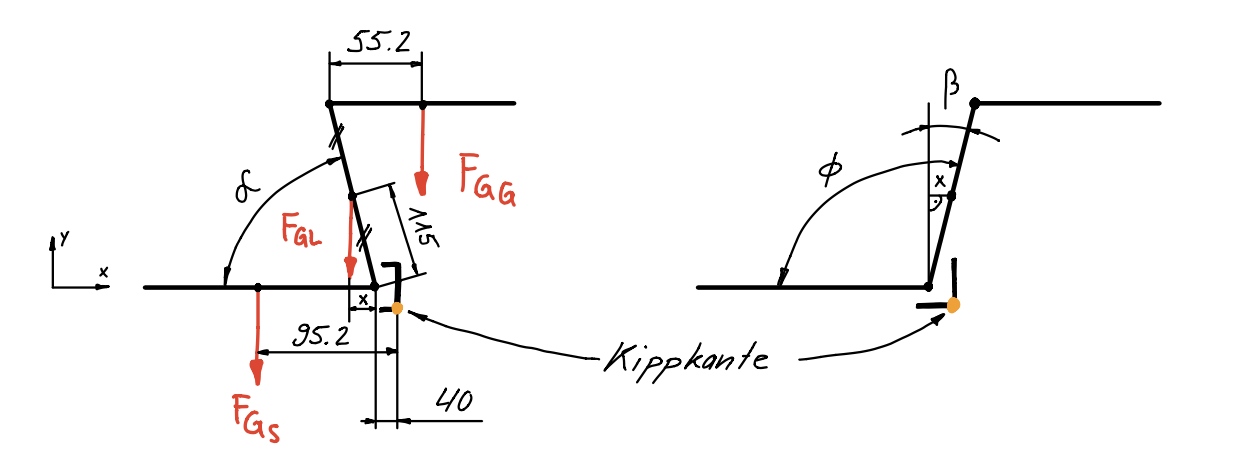
\includegraphics[width=1\textwidth]{img/Treppensteigen/Standsicherheit 1.Hub.png}
  \centering
  \caption{Skizze Standsicherheit bei der 1. Hubbewegung}
\end{figure}

Standsicherheit ist bis {\alpha} = 90$^\circ$ gegeben.

Für {\alpha} = 90$^\circ$ gilt:

\begin{align*}
    M_{Stand} &= F_{GS} * 140\ mm + F_{GL} * 40\ mm \\
    &= g\ (m_{Standfuesse} * 140\ mm + m_{Verbindungsleisten} * 40\ mm) \\
    &= 9.81\ m/s^2\ * (0.6\ kg * 140\ mm + 0.4\ kg * 40\ mm) \\
    &= \underline{\underline{0.9\ Nm}}
\end{align*}

\begin{align*}
    M_{Kipp} &= F_{GG} * 10\ mm \\
    &= g\ (m_{Grundkoerper} * 10\ mm) \\
    &= 9.81\ m/s^2\ * (2\ kg * 10\ mm) \\
    &= \underline{\underline{0.2\ Nm}}
\end{align*}

Daraus folgt:
\[M_{Stand} > M_{Kipp}\]

\newpage
Für {\alpha} > 90$^\circ$ gilt:

\begin{align*}
    F_{GS} * 140\ + F_{GL} * (40\ - x) &= (50\ + 2x\ - 40)\ \text{wenn}\ x < 40 \\
    m_{S} * g * 140 + m_{V} * g * (40 - x) &= m_{G} * g * (10 + 2x) \\
    m_{S} * 140 + m_{V} * 40 - m_{V} * x &= m_{G} * 10 + m_{G} * 2x \\
    (2 * m_{G} + m_{V}) x &= m_{S} * 140 + m_{V} * 40 - m_{G} * 10 \\
    x &= (m_{S} * 140 + m_{V} * 40 - m_{G} * 10)\ /\ (2 * m_{G} + m_{V}) \\
    x &= 18.2\ mm\ (\text{erfüllt}\ x < 40 mm)
\end{align*}


\({\beta} = \arcsin{(18.2\ mm\ /\ 115\ mm)} = 9.1^{\circ} \)

\({\phi} = 90^{\circ} + {\beta} = 90^{\circ} + 9.1^{\circ} = 99.1^{\circ} \)

Bei der ersten Hubbewegung ist die Standsicherheit bis {\phi} = 99.1$^\circ$ gegeben.


\textbf{2.Hubbewegung:}

\begin{figure}[H]
  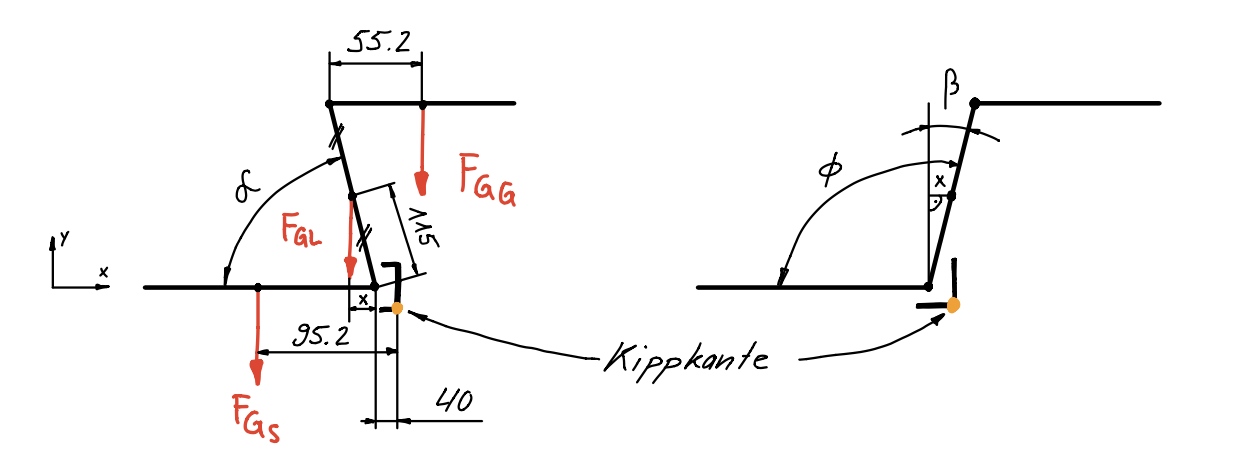
\includegraphics[width=1\textwidth]{img/Treppensteigen/Standsicherheit 1.Hub.png}
  \centering
  \caption{Skizze Standsicherheit bei der 2. Hubbewegung}
\end{figure}

Wenn die Standfüsse bei der 2.Hubbewegunng waagrecht gehalten werden, ist die kritische Stelle der Hubbewegung, wenn die Standfüsse und die Verbindungsleisten in einer Linie mit dem Drehpunkt des Grundkörpers sind.

In diesem Fall gilt:

\begin{align*}
    M_{Stand} &= F_{GG} * 100\ mm \\
    &= g * m_{Grundkoerper} * 100\ mm \\
    &= 9.81\ m/s^2\ * 2\ kg * 100\ mm \\
    &= \underline{\underline{1962\ Nmm}}
\end{align*}

\begin{align*}
    M_{Kipp}  &= F_{GS} * (230\ mm + 100\ mm - 50\ mm) + F_{GL} * (115\ mm - 50\ mm) \\
    &= g * (m_{Standfuesse} * 280\ mm + m_{Verbindungsleisten} * 65\ mm) \\
    &= 9.81\ m/s^2\ (0.6\ kg * 280\ mm + 0.4\ kg * 65\ mm) \\
    &= \underline{\underline{1903\ Nmm}}
\end{align*}
  
Daraus folgt:
\[M_{Stand} > M_{Kipp}\]

\subsubsection{1. Hubbewegung Analyse}
\label{HubbewegungAnalyse}

Mit den ersten Massabschätzungen und der ersten Platziervorstellung auf dem aktuellen Treppentritt wurde berechnet, ob der Grundkörper bei der ersten Hubbewegung mit der Kante des des nächsten Treppentrittes kollidert oder nicht. Es wurde auch berechnet, auf welcher Höhe über dem nächsten Treppentritt und wie weit über der Kante des nächsten Trittes sich der Grundkörper beim kritischen Kippwinkel befindet.

\begin{figure}[H]
  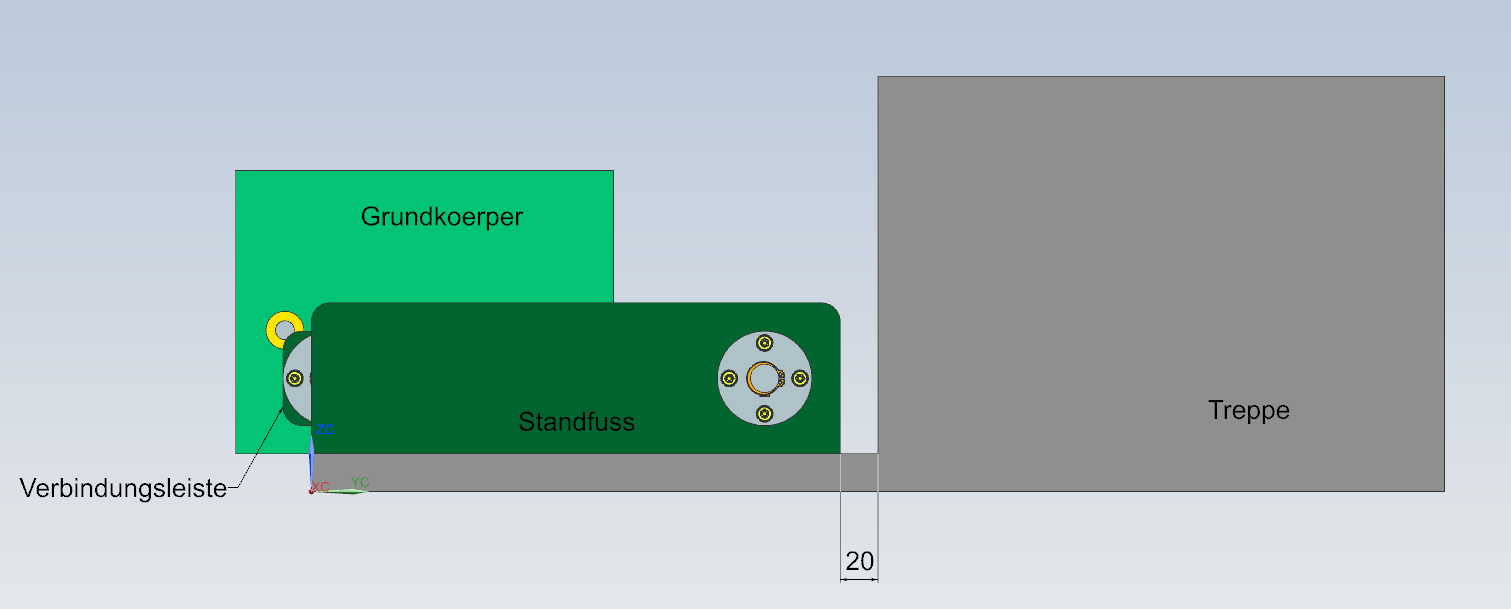
\includegraphics[width=1\textwidth]{img/Treppensteigen/Platzierung auf Treppe.PNG}
  \centering
  \caption{Platzierung auf aktueller Treppenstufe vor 1. Hubbewegung}
\end{figure}

\textbf{Kritischer Kippwinkel erreicht}

Beim Start der 1. Hubbewegung ist die vordere Kante des Geräts 20 mm von der nächsten Trittkante entfernt. Im Ausgangszustand ist der Grundkörper 140 mm vom nächsten Tritt entfernt.\\

\begin{figure}[H]
  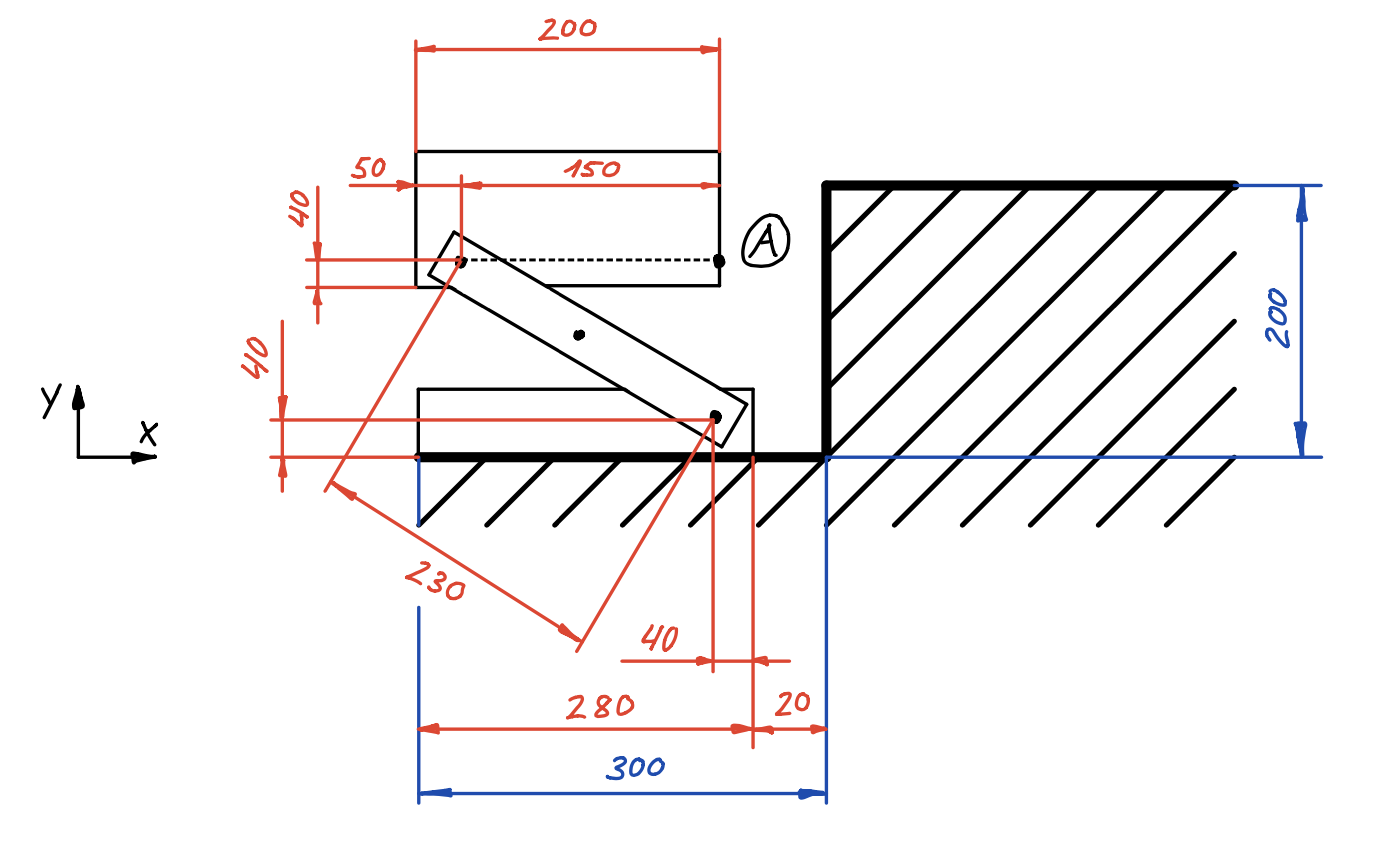
\includegraphics[width=0.8
  \textwidth]{img/Treppensteigen/Skizze Platzierung}
  \centering
  \caption{Skizze Platzierung mit Massen}
\end{figure}

\begin{figure}[H]
  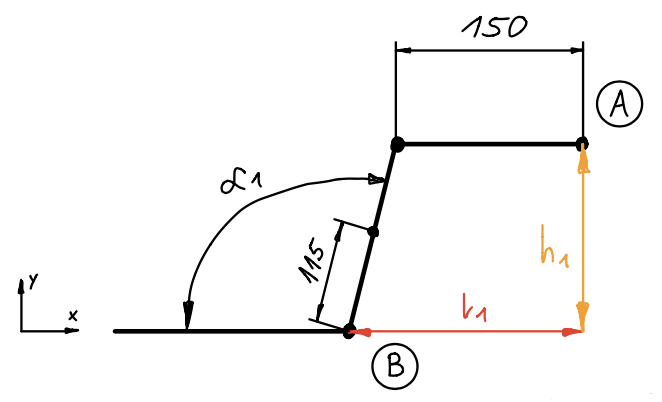
\includegraphics[width=0.6
  \textwidth]{img/Treppensteigen/Analyse 1.png}
  \centering
  \caption{Skizze kritischer Kippwinkel erreicht}
\end{figure}

Der betrachtete Punkt A befindet sich horizontal auf der gleichen Höhe wie der obere Drehpunkt. Im Ausgangszustand ist Punkt A 140 mm in X-Richtung vom nächsten Tritt entfernt. Der Drehpunkt B ist in X-Richtung 60 mm vom nächsten Tritt entfernt.

Wo befindet sich Punkt A, wenn der kritische Kippwinkel \alpha$_{1}$ = 99.1$^\circ$ erreicht ist?

l$_{1}$ = 150 mm + 230 mm * sin(\alpha$_{1}$ - 90$^\circ$) = 186. 4 mm

Punkt A in X-Richtung über nächster Trittkante = 186.4 mm - 60 mm = 126.4 mm

Somit ist auch die Kante des Grundkörpers 126.4 mm in X-Richtung über nächster Trittkante.\\

h$_{1}$ = 230 mm * cos(\alpha$_{1}$ - 90$^\circ$) = 227.1 mm

Somit ist die Kante des Grundkörpers in Y-Richtung 27.1 mm über der nächsten Trittkante.\\
\\

\textbf{Kante des Grundkörpers über Treppenkante}

Wenn die Kante des Grundkörpers in X-Richtung auf gleicher Höhe wie die nächste Trittkante ist, welchen Abstand hat dann die Kante des Grundkörpers in Y-Richtung?\\

\begin{figure}[H]
  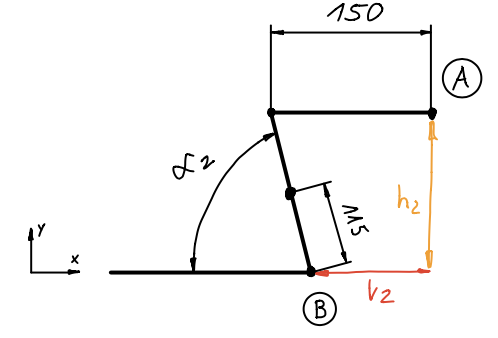
\includegraphics[width=0.6\textwidth]{img/Treppensteigen/Analyse 2.png}
  \centering
  \caption{Skizze Punkt A in X-Richtung auf Höhe der nächsten Trittkante}
\end{figure}

l$_{2}$ = 60 mm

\alpha$_{2}$ = arccos((150 mm - l$_{2}$) / 230 mm) = 67$^\circ$

h$_{2}$ = 230 mm * sin(\alpha$_{2}$)  = 211.7 mm

Die Kante des Grundkörpers in Y-Richtung ist 11.7 mm über der nächsten Trittkante wenn Punkt A in X-Richtung auf gleicher Höhen wie die nächste Trittkante ist.\\


\subsubsection{Benötigte Momente}

Die Momente, die gebraucht werden, konnten mit den ersten Gewichts- und Massabschätzungen berechnet werden und dienen als Motorenauswahl Grundlage.

\newpage

\textbf{Momente bei den Hubbewegungen:}

\textbf{1. Hubbewegung:}

Drehachse 1: Moment zu horizontalen Halten des Grundkörpers
\begin{align*}
    M_{Achse 1} &= F_{GG} * 0.06\ m \\
    &= m_{GG} * g * 0.06\ m \\
    &= 2\ kg * 9.81\ m/s^2\ * 0.06\ m \\
    &= \underline{\underline{1.2\ Nm}}
\end{align*}

Drehachse 2: grösstes Moment am Anfang, in Ausgangsstellung
\begin{align*}
    M_{Achse 2} &= F_{GL} * 0.115\ m + F_{GG} * 0.23\ m \\
    &= g * (m_{GL} * 0.115\ m + m_{GG} * 0.23\ m \\
    &= 9.81\ m/s^2\ * (0.4\ kg * 0.115\ m + 2\ kg * 0.23\ m) \\
    &= \underline{\underline{5\ Nm}}
\end{align*}

\textbf{2. Hubbewegung:}

Drehachse 1: grösstes Moment, wenn alle Teile horizontal
\begin{align*}
    M_{Achse 1} &= F_{GS} * 0.33\ m + F_{GL} * 0.115\ m \\
    &= g * (m_{GS} * 0.33\ m + m_{GL} * 0.115\ m) \\
    &= 9.81\ m/s^2 * (0.6\ kg * 0.33\ m + 0.4\ kg * 0.115\ m) \\
    &= \underline{\underline{2.4\ Nm}}
\end{align*}

Drehachse 2: grösstes Moment, wenn Standfüsse horizontal
\begin{align*}
    M_{Achse 2} &= F_{GS} * 0.1\ m \\
    &= m_{GS} * g * 0.1\ m \\
    &= 0.6\ kg * 9.81\ m/s^2 * 0.1\ m \\
    &=\underline{\underline{0.6\ Nm}}
\end{align*}

Motor 1 liefert das Moment, das in der 1. Drehachse wirkt und Motor 2 liefert das Moment, das in der 2. Drehachse wirkt.\\
\\
M$_{erforderlich}$ Motor 1: 5 Nm\\

M$_{erforderlich}$ Motor 2: 2.4 Nm

\newpage
\subsection{Elektrotechnisches Konzept}
\subsubsection{Auslegung Elektromotoren}
Der erste Motor benötigt gemäss Berechnungen ein maximales Drehmoment von 5 Nm. Dazu passt der Getriebemotor Modelcraft IG320516-41C01 von conrad \cite{Getriebemotor1}. Dieser liefert ein maximales Drehmoment von 4.2 Nm. 
Der zweite Motor benötigt gemäss Berechnungen ein maximales Drehmoment von 2.4 Nm. Dazu passt der Getriebemotor Modelcraft RB350600-0A101R ebenfalls von conrad \cite{Getriebemotor2}. Dieser liefert ein maximales Drehmoment von 3.2 Nm.

\subsubsection{Sensorik für die Bewegungen}
Die Bewegungen werden durch Elektrogetriebemotoren umgesetzt. Damit die Steuerung die Bewegungen autonom ausführen kann, benötigt die Steuerung Rückmeldungen, in welcher Position sich der Grundkörper und die Standfüsse befinden. Dies soll mittels Tastsensoren realisiert werden.

\begin{figure}[h]
  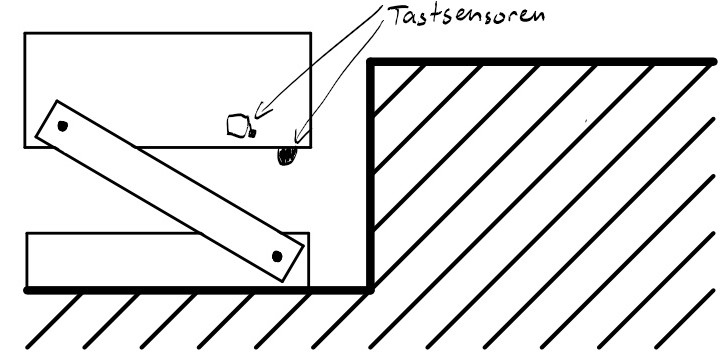
\includegraphics[width=0.6\textwidth]{img/Treppensteigen/Sensoren_Treppensteigen2.png}
  \centering
  \caption{Platzierung der Tastsensoren für die Bewegungen}
  \label{fig2}
\end{figure}

Die Abbildung \ref{fig2} zeigt an welchem Ort der Komponenten die Tastsensoren angebracht werden sollen. Der erste Tastsensor befindet sich unterhalb des Grundkörpers und gibt Rückmledung, ob der Grundkörper den Boden berührt. Der zweite Tastsensor befindet sich seitlich am Grundkörper und gibt Rückmeldung, wenn sich die Verbindungsleisten am Grundkörper befinden. Wenn sich der Roboter im Ausgangszustand befindet (eingefahren) sind beide Sensoren aktiv. Danach wird die erste Hubbewegung so lange ausgeführt beziehungsweise der Motor angesteuert, bis sich der Grundkörper auf der Treppe befindet und sich der untere Sensor aktiviert. Danach wird der Motor für die zweite  Hubbewegung solange angesteuert, bis sich die Verbindungsleisten wieder am Grundkörper befinden und die seitlichen Sensoren wieder aktiv sind.


Bei den Hubbewegungen muss der Grundkörper gerade gehalten werden:
\begin{itemize}
    \item Um in der ersten Hubbewegung der Grundkörper gerade halten zu können, wird ein Drehmoment von 1.2 Nm benötigt. Gemäss Datenblatt des Elektromotors IG320516-41C01 gibt der Motor bei einem Strom von 0.5 A und einer Leistung von 1.51 W ein Drehmoment von 1.31 Nm ab. Daraus folgt eine Spannung von 3 V, welche mit einer H-Brücke eingestellt wird.
    \item Das Prinzip der zweiten Hubbewegung ist analog zur Ersten. Der Elektromotor RB350600-0A101R gibt gemäss Datenblatt bei einem Strom von 0.2 A und einer Leistung von 0.51 W ein Drehmoment von 0.6 Nm ab. Daraus folgt eine Spannung von 2.55 V.
 \end{itemize}


\newpage
\subsection{Fortbewegung}
Die horizontale Fortbewegung wird mit zwei, unabhängigen voneinander angetriebenen Rädern ermöglicht. Zusätzlich zu diesen zwei Rädern werden zwei Stützpunkte benötigt, damit der Grundkörper nicht den Boden berührt. Verwendet werden zwei, damit bei der Roboter bei der Hubbewegung auf die nächste Stufe gerade bleibt. Diese Stützpunkte werden auf einem Tastsensor (vergleich Sensorik für die Bewegung) montiert und sind in der Form einer Halbkugel, um einfaches gleiten zu gewährleisten und sicherzustellen, dass der Stützpunkt auf der Treppe nicht hängen bleibt.

\begin{figure}[H]
  \includegraphics[width=0.8\textwidth]{img/Fortbewegung/Skizze Räder.png}
  \centering
  \caption{Skizze Räder mit Halbkugelstützen}
\end{figure}

Dieses Fortbewegungsprinzip ermöglicht es dem Gerät, sich an Ort und Stelle zu drehen, indem die Räder entgegegesetzt angesteuert werden. Das Gerät kann sich somit im Start- und Zielbereich in alle Richtungen bewegen. Dies ist zu Beginn, für das Fahren vor die Treppe und zum Schluss, beim Suchen des Zielpiktogramms vorteilhaft. Um auf den Treppenstufen nach links oder rechts auszuweichen, soll sich das Roboter zuerst um 90$^\circ$ drehen, dann geradeaus fahren und sich anschliessend wieder um 90$^\circ$ drehen, sodass sich das Gerät an der Position für den nächsten Treppensteigprozess rechtwinklig vor dem nächsten Treppentritt befindet.

\newpage

\subsubsection{Berechnung der Antriebsleistung}

Für eine erste Berechnung der notwendigen Antriebsleistung zur Fortbewegung wurde ein Raddurchmesser und eine maximale Wunscheschwindigkeit angenommen. Die Räder sollen aus Gummi sein. Die Materialien, die das Gerät befahren muss sind Holz im Startbereich und Aluminium auf der Treppe. Für die Berechnung des notwendigen Antriebsmoments auf Holz und Aluminium, ohne durchrutschen der Räder, wird ein Reibungskoeffizent \cite{Reibung} für die Paarung Gummi-Metall verwendet. Wird das gleiche berechnete Moment auf der Holzunterlage aufgebracht, ist das durchrutschen weniger kritisch, da die Reibung zwischen dem Holz und den Gummirädern grösser ist.

\begin{figure}[H]
  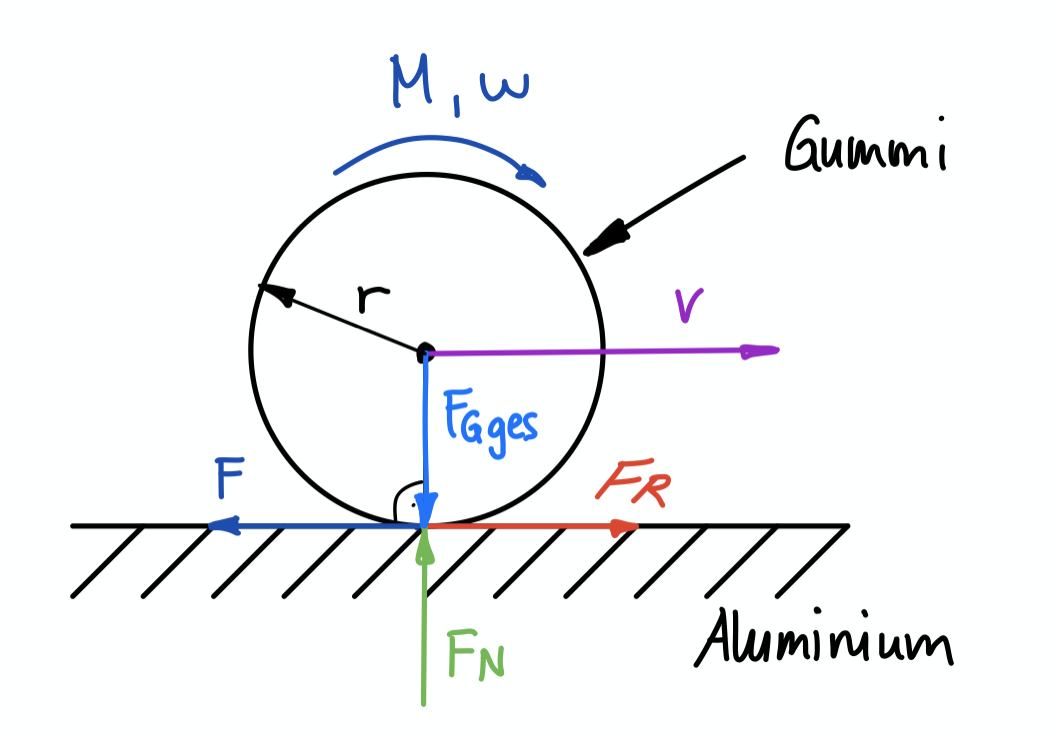
\includegraphics[width=0.8\textwidth]{img/Fortbewegung/Radberechnung.png}
  \centering
  \caption{Skizze zur Radberechnung}
\end{figure}

\newpage

Betrachtet wird ein Rad. Ein Rad trägt ungefähr 1/4 des Gesamtgewichts.

m$_{ges}$ = 3 kg

d$_{Rad}$ = 80 mm

v$_{Wunsch}$ = 2 m/s

\( \mu_{Gummi-Aluminium} = 0.5\)

\[F_{Gges} = m_{ges} * g = 3\ kg * 9.81\ m/s^2\ = 29.4\ N \]

\[F_N = F_{Gges}\ /\ 4 = 29.4\ N\ /\ 4 = 7.35\ N \]

\[F = F_R = F_N * {\mu_{Gummi-Aluminium}} = 7.35\ N * 0.5 = 3.68\ N\]

\[M_{max} = F * r = 3.68\ N * 0.04\ m = 0.015\ Nm\]

\[\text{Kein Rutschen}: \omega_{max} = v_{Wunsch}\ /\ r = 2\ m/s\ /\ 0.04\ m = 50\ rad/s\]


\subsubsection{Auswahl der Motoren für die Fortbewegung}
Für die Fortbewegung am Boden benötigt der Roboter 2 Motoren. Gemäss Berechnung benötigt je ein Motor ein Drehmoment von 0.015 Nm. Zusätzlich sollen die Motoren mit einem Encoder ausgestattet sein, um eine 90\textdegree-Drehung ausführen zu können bzw. um den zurückgelegten Weg ermitteln zu können. Eine Auswahl für diesen Motortyp ist der DC 12 V DIY Encoder Getriebemotor von amazon \cite{MotorEncoder}. Dieser liefert ein maximales Drehmoment von 0.9 Nm. 
Die Funktion eines Encoders oder Inkrementalgeber kann wie folgt beschrieben werden: Ein Inkrementalgeber hat 2 Ausgangssignale \glqq A\grqq{} und \glqq B\grqq{}. Die Abbildung \ref{fig4} zeigt den zeitlichen Verlauf der Kanäle. Ein Signal ist jeweils um 90\textdegree\ versetzt. Durch Drehen des Drehgebers im Uhrzeigersinn, wird der \glqq A\grqq{} Puls um 90\textdegree{} vor dem \glqq B\grqq{} Puls gesendet. Durch Drehen der Welle gegen den Uhrzeigersinn wird der \glqq B\grqq{} Puls vor dem \glqq A\grqq{} Puls gesendet. Dadurch kann per Software die Drehrichtung und die Geschwindigkeit ermittelt werden.

\begin{figure}[H]
  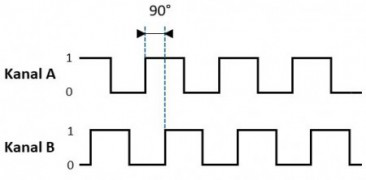
\includegraphics[width=0.6\textwidth]{img/Fortbewegung/Increment Encoder Signal.png}
  \centering
  \caption{Kanal A und B eines Inkrementalgebers}
  \label{fig4}
\end{figure}


\subsubsection{Überwachung der Fortbewegung}

TODO Sensoren für Überwachung der Fortbewegung

\newpage
\subsection{Elektrosteuerung}
Die Steuerung der Elektrokomponenten wie Motoren, Sensoren und Kameras erledigt ein Raspberry Pi. Das Bord steuert nicht nur die Eingänge, der Sensoren und steuert die Motoren an, sondern es verarbeitet die Bilder und berechnet das Pathfinding. Das Raspberry Pi ist das Gehirn des Roboters.

\subsubsection{Kapazität Akku}
Die elektrischen Komponenten des Roboters werden mit Energie versorgt. Diese Energie soll ein LiPo-Akku liefern. Um die Kapazität grob bestimmen zu können werden die Verbräuche der Komponenten aufgelistet:   

\begin{table}[h!]
\centering
\begin{tabular}{ l l }
 \textbf{Komponenten} & \textbf{Leistung (max)} \\
 2x TOF-Abstandssensoren & 0.04 W \\ 
 Motor 1+2 Treppensteigen & 4.39 W \\  
 Motor 1+2 Fortbewegung & 5 W \\
 Raspberry Pi 3 mit Kamera & 3 W \\
 4x H-Brücken & 0.2 W \\
 \textbf{Total} & \textbf{12.63 W}
\end{tabular}
\caption{Stromverbrauch der Komponenten}
\end{table}

Der Roboter muss gemäss Anforderungskatalog 12 min fahren können. Die Energie lässt sich wie folgt berechnen:
\[E = P * t = 12.63\ W * \frac{12\ min}{60} = 2.526\ Wh\]
Daraus lässt sich die Kapazität berechnen:
\[C = \frac{E}{U} = \frac{2.526\ Wh}{12\ V} * 1000 = 210\ mAh\]
Ein dazu passender Akku mit genügend Reserven ist der Tattu Modellbau-Akkupack (LiPo) 14.8 V 650 mAh von conrad \cite{Akku}.


\newpage
\subsection{Umgebungserkennung}
\subsubsection{Orientierung}
\textbf{Finden des Piktogramms im Startfeld}\\
Um im Startfeld das Piktogramm zu finden wird die Kamera verwendet. Hier ist geplant, mit einem FindContours-Algorithmus \cite{OpenCV-Fining-Contours} in OpenCV alle Konturen mit vier Eckpunkten herauszufiltern. Dabei werden diese gefundenen Konturen mit vier Eckpunkten nach der Grösse der Fläche sortiert. Dabei wird davon ausgegangen, dass die grösste dieser Konturen das Schild mit dem Piktogramm ist. Es wird angenommen, dass es plausibel ist, dass das grösste Objekt mit genau vier Eckpunkten und Kanten, das Schild mit dem Piktogramm ist.\\ 
Sobald eine plausible Kontur gefunden wurde kann das Bild bereits für die Piktogrammerkennung vorbereitet werden. Hierbei wird es auf die Region of Interes (ROI) begrenzt und optional mit der getGeometricTransform-Methode von OpenCV eine Top-Down-View auf das Bild erstellt. Da es sich bei den Piktogrammen um Schwarz-Weiss-Bilder handelt, kann man hier noch leicht die unterschiedlichen Lichtverhältnisse herausfiltern, in dem man noch eine Threshold anwendet.
Folgend eine Auflistung der geplanten Bildverarbeitungsschritte:
\begin{enumerate}
    \item Verkleinerung
    \item In Graustufen konvertieren 
    \item Verzerren
    \item Erkennen von Kanten (Canny edge detection)
    \item Finden der Konturen
    \item Sortieren aller Rechteckigen Konturen nach Fläche
    \item Einzeichnen der Konturen mit grösster Fläche auf dem Originalbild
    \item Auf ROI zuschneiden
    \item Optional: Top-Down-View auf das Bild erstellen (getGeometricTransform())
    \item Thresholding
\end{enumerate}

\textbf{Finden der Treppe im Startfeld}\\
Für das Finden der Treppe soll der gleiche Algorithmus verwendet werden, mit welchem auch das Path-Finding realisiert werden soll. Sobald also das Piktogramm gefunden und der Auftrag quittiert wurde, macht sich der Roboter auf die Suche nach der Treppe. Danach fährt der Roboter an den Start des definierten Pfades. Damit die Ausrichtung zur Treppe genau 90° Beträgt, ist der Roboter mit zwei Distanzsensoren an der Vorderseite ausgestattet. Die beiden gemessenen Distanzen zur ersten Treppenstufe können so gleich gehalten werden.

\textbf{Ausrichtung zur Treppe}
Um eine Treppenstufe erfolgreich erklimmen zu können, muss der Roboter genau senkrecht zur Treppe stehen. Um dies zu gewährleisten stehen folgende Möglichkeiten zur Verfügung:
\begin{enumerate}
    \item \textbf{Tastsensor}\\
    Der Roboter ist mit zwei Tastsensoren ausgestattet, welche sich auf gleicher Höhe mit der Stufe befinden. Diese triggern sobald der Roboter genügend stark gegen die Treppe fährt. Der Roboter fährt so lange gegen die Treppe, bis beide Tastsensoren detektieren. Über den Tastsensoren soll ein Puffer befestigt werden, damit die Kraft präziser übertragen wird.
    
    \textbf{Vorteile}
    \begin{itemize}
        \item Bereits mit sehr wenig Geld erhältlich.
        \item Sehr simpel.
    \end{itemize}
    \textbf{Nachteile}
    \begin{itemize}
        \item Eine fixe Schwelle der Kraft, welche aufgewendet werden muss, damit der Taster detektiert.
        \item Muss sich genau auf der Höhe der Treppenstufe befinden.
    \end{itemize}
    
    \item \textbf{Kraftsensor}\\
    Mit den Kraftsensoren wird das selbe Prinzip wie mit den Tastsensoren verfolgt. Der Vorteil hierbei ist, dass diese im Gegensatz zu den Tastsensoren schon sehr schwache "Kollisionen" mit der Treppenstufe detektieren. Somit wird mit einer höheren Genauigkeit gerechnet. Wobei sie preislich etwas teurer sind.
    
    \textbf{Vorteile}
    \begin{itemize}
        \item Detektieren bereits sehr schwache Kollisionen.
    \end{itemize}
    \textbf{Nachteile}
    \begin{itemize}
        \item Sind teurer als die Tastsensoren.
        \item Muss sich genau auf der Höhe der Treppenstufe befinden.
    \end{itemize}
    
    \item \textbf{Tast- oder Kraftsensoren mit ausfahrbaren Fühler}\\
    Der Roboter darf sich jedoch nicht unmittelbar vor der Treppenstufe befinden, um die Hubbewegung durchzuführen (siehe \ref{HubbewegungAnalyse}), da die Treppenstufe sonst im Weg steht. Somit kann der Roboter Fühler ausfahren, an welchen die Tast- bzw. Kraftsensoren befestigt sind, welche den Roboter genau auf der richtigen Distanz halten. Die Fühler werden vor der Hubbewegung ein wenig eingefahren, so dass die Treppe nicht mehr blockiert.
    
    \textbf{Vorteile}
    \begin{itemize}
        \item Der Roboter kann einfach gegen die Treppe fahren und richtet sich so automatisch senkrecht aus.
    \end{itemize}
    \textbf{Nachteile}
    \begin{itemize}
        \item Auwändig und tuer
        \item KISS-Prinzip nicht eingehalten
        \item Genauigkeit sehr von der verwendeten Technologie (z.B. Servo) fürs Einfahren der Fühler
        abhängig. 
        \item Muss sich genau auf der Höhe der Treppenstufe befinden.
    \end{itemize}
    
    \item \textbf{Zwei Kameras}\\
    Mithilfe von zwei unabhängigen Kameras sollen die Diszanzen zur Treppe gemessen werden. Wenn beide Distanzen gleich sind, steht der Roboter senkrecht zur Treppe.
    
    \textbf{Vorteile}
    \begin{itemize}
        \item Die Kameras müssen sich nicht auf gleicher Höhe wie die Treppenstufe befinden.
    \end{itemize}
    \textbf{Nachteile}
    \begin{itemize}
        \item Komplex
        \item Ungenau
        \item Preis
    \end{itemize}
    
    \item \textbf{Distanzsensoren}\\
    Mit den Distanzsensoren wird das selbe Prinzip wie mit den Kameras verfolgt. Sie sollen die Distanz zur nächsten Treppenstufe messen.
    
    \textbf{Vorteile}
    \begin{itemize}
        \item Günstig
    \end{itemize}
    \textbf{Nachteile}
    \begin{itemize}
        \item Muss sich genau auf der Höhe der Treppenstufe befinden.
    \end{itemize}
\end{enumerate}
\textbf{Fazit:} Die Tastsensoren und Kraftsensoren fallen raus, aufgrund der Hubbewegung. Die ausfahrbaren Fühler fallen aufgrund des Entwicklungsaufwandes heraus. Die zwei Kameras aufgrund des Preises, der Komplexität und der ungenügenden Genauigkeit. Der Roboter wird also mit zwei Distanzsensoren ausgestatten, mit welchen die Ausrichtung zur Treppe sichergestellt werden kann.
\image
   {img/orientierung-treppenstufe/Distanzsensoren.png}
   {Skizze der Befestigungspunkte der Distanzsensoren}


\textbf{Orientierung auf der Treppenstufe}\\
Um sich auf einer Treppenstufe orientieren zu können, ist geplant mithilfe eines Linefollowing Algorithmus der Treppenstufe sicher entlang zu fahren. Ebenfalls ist gedacht, den Linefollowing Algorithmus dazu zu verwenden, die Ausrichtung des Roboters auf der Treppenstufe zu kontrollieren (siehe Kapitel \ref{orientierungAufTreppenstufe}).
Die zurückgelegte Distanz auf einer Treppenstufe soll mithilfe des Encoders der Motoren berechnet werden.

\subsubsection{Hindernisserkennung}
TODO
\subsubsection{Piktogrammerkennung}
Erst war geplant, die Piktogrammerkennung mit einem Convolutional Neural Network (CNN) zu realisieren. Hierbei wird ein Modell darauf trainiert, die fünf Piktogramme zu erkennen. Während der Erstellung des Funktionsmusters (siehe Kapitel \ref{piktogrammerkennungMitCNN}) und den Weekly-Standups mit dem Coach hat sich herausgestellt, dass es passendere Techniken gibt.\\
Da es sich um ein endliches Problem handelt, weil man lediglich fünf verschiedene Piktogramme erkennen und unterscheiden muss, war der zweite Lösungsansatz sogenanntes Template Matching\cite{OpenCV-Template-Matching}. Bei der Recherche hat sich herausgestellt, dass diese Methode gute Resultate liefert, wenn man lediglich mit Translationen und Skalierungen zu tun hat. Sobald das Bild, in dem das Piktogramm detektiert werden soll, Rotationen und nicht affine Transformationen aufweist, ist man besser dran mit Keypoint Detection, Image Deskriptoren und Keypoint Matching\cite{OpenCV-Feature-Matching}. Aus diesem Grund ist geplant die Piktogrammerkennung mit letzterem umzusetzen.




\subsection {Kommunikation}

Um das Finden und Verarbeiten des Piktogramms sowohl im Start- als auch im Zielbereich zuverlässig und einfach zu signalisieren, werden zwei verschiedene Methoden verwendet. Einerseits die Visualisierung mittels LEDs und anderseits die auditive Quittierung. Diese Audiowiedergabe wird entweder mittels Buzzer, oder mittels eines Lautsprechers getätigt. Die Visualisierung mittels LEDs erfolgt über das Raspberry selbst.

Die Audiowiedergabe über den Buzzer ermöglicht einfache Tonabfolgen und wird über die Spannung eines Pins gesteuert. Das Prinzip ist einfach und schnell, ist bezüglich der Lautstärke und dem \glqq WoW-Effekt \grqq{} dem Lautsprecher jedoch deutlich unterlegen.
Die Ausgabe über die USB-Lautsprecher erfolgt direkt über das Raspberry. Die Speaker werden direkt mittels USB und der 3.5mm Klinke mit dem Raspberry verbunden. Mit wenigen Zeilen Code kann so ein vollwertiges Audiofile abgespielt werden.
Die Lautsprecher sind in jeglicher Hinsicht besser und einfacher mit der Ausnahme des Platzbedarfs. Ist der Platz und das Gewicht verfügbar, werden die Lautsprecher verbaut 

\newpage
\subsection{Zusammenspiel der Teilfunktionen}
 Die Abbildung \ref{fig3} zeigt das Blockschaltbild des Zusammenspiels der Teilfunktionen.

\begin{figure}[h]
  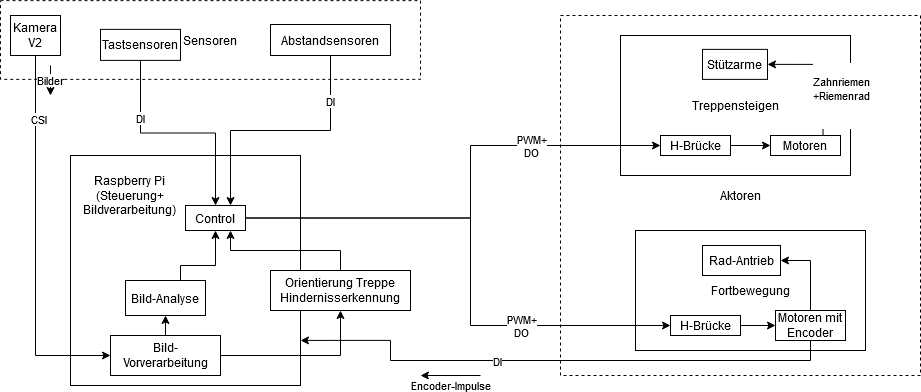
\includegraphics[width=\textwidth]{img/Funktionsmuster Treppensteigen/Blockschaltbild.png}
  \centering
  \caption{Blockschaltbild der Prozesse Elektrotechnik/Mechanik}
  \label{fig3}
\end{figure}

 Das Blockschaltbild zeigt als zentrale Steuerungseinheit einen Raspberry Pi. Dieser übernimmt die Aufgabe der Bildverarbeitung für die Orientierung auf der Treppe sowie für die Hinderniserkennung. Diese Informationen verarbeitet die Steuerung und gibt entsprechende Signale an die Aktoren weiter. Zu den Aktoren gehören die Elektromotoren inkl. H-Brücken für die Ansteuerung, sowie die mechanischen Komponenten für das Treppensteigen und die Fortbewegung. Die Elektromotoren der Fortbewegung senden ein Encodersignal zurück an den Raspberry Pi. Zu den Sensoren des Konzeptes gehören Kameras, die Bilder für die Bildverarbeitung liefern. Zusätzlich liefern Abstands- und Tastsensoren für die Orientierung und das Treppensteigen Inputsignale für die Steuerung.
 
 \subsubsection{Schnittstellenbeschreibung}
TODO Yves